\chapter{需求建模 }
\section{数据流图}
\subsection{顶层数据流图}
在这里画出顶层数据流图
\begin{figure}[ht]
	\centering
 	\includegraphics[scale=0.5,bb=0 0 1920 1080]{lv-00}
	\caption{顶层数据流图} 
	\label{fig:figure11}
\end{figure}

\subsection{0层数据流图}
\begin{figure}[ht]
	\centering
	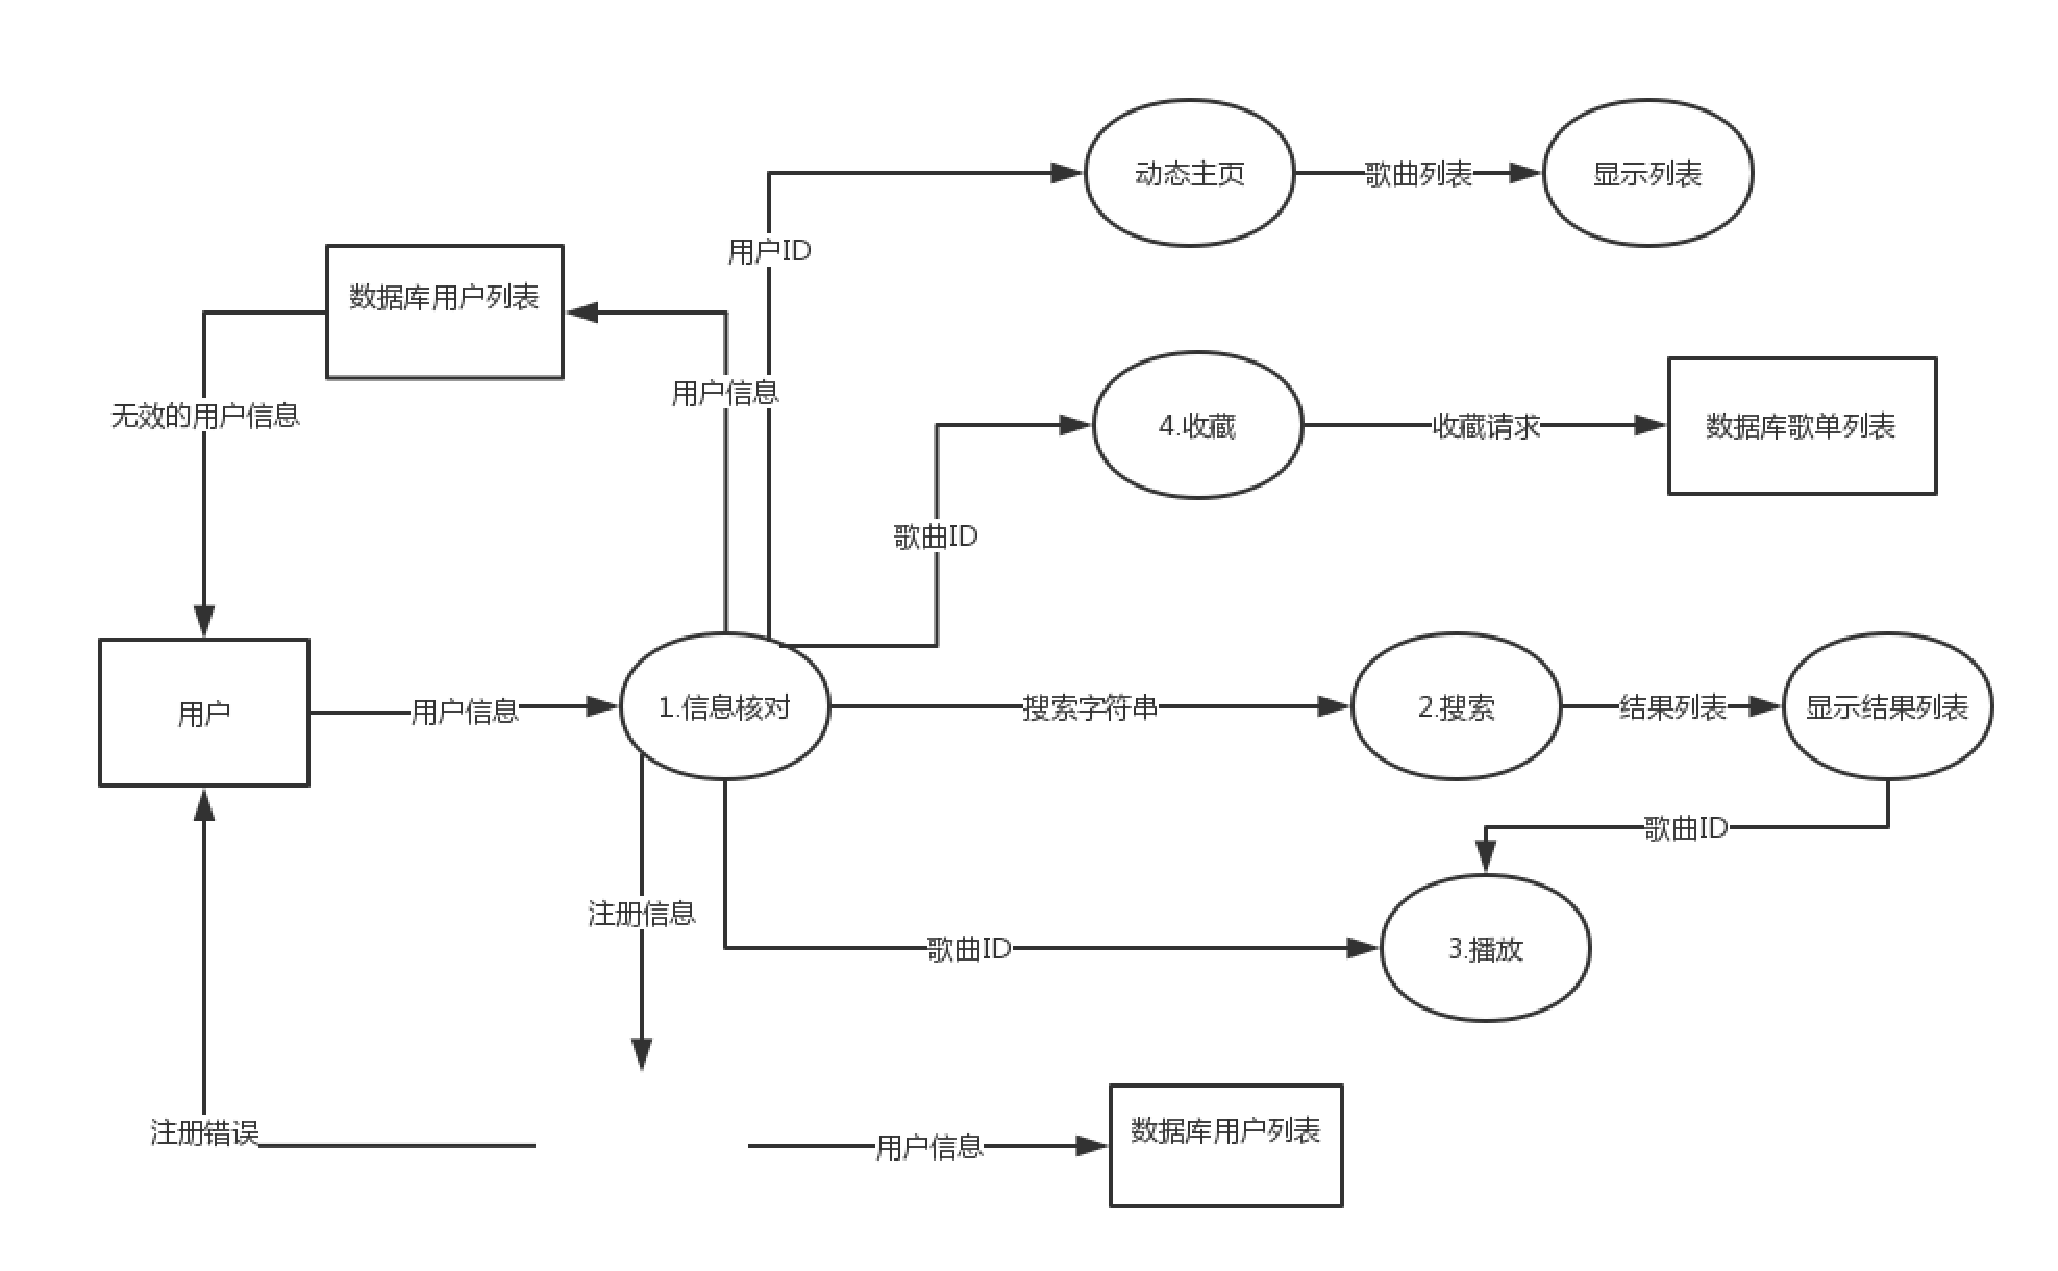
\includegraphics[width=10cm]{lv-0}
	\caption{0层数据流图} \label{fig:figure12}
\end{figure}

\subsection{1层数据流图}
\begin{figure}[ht]
	\centering
	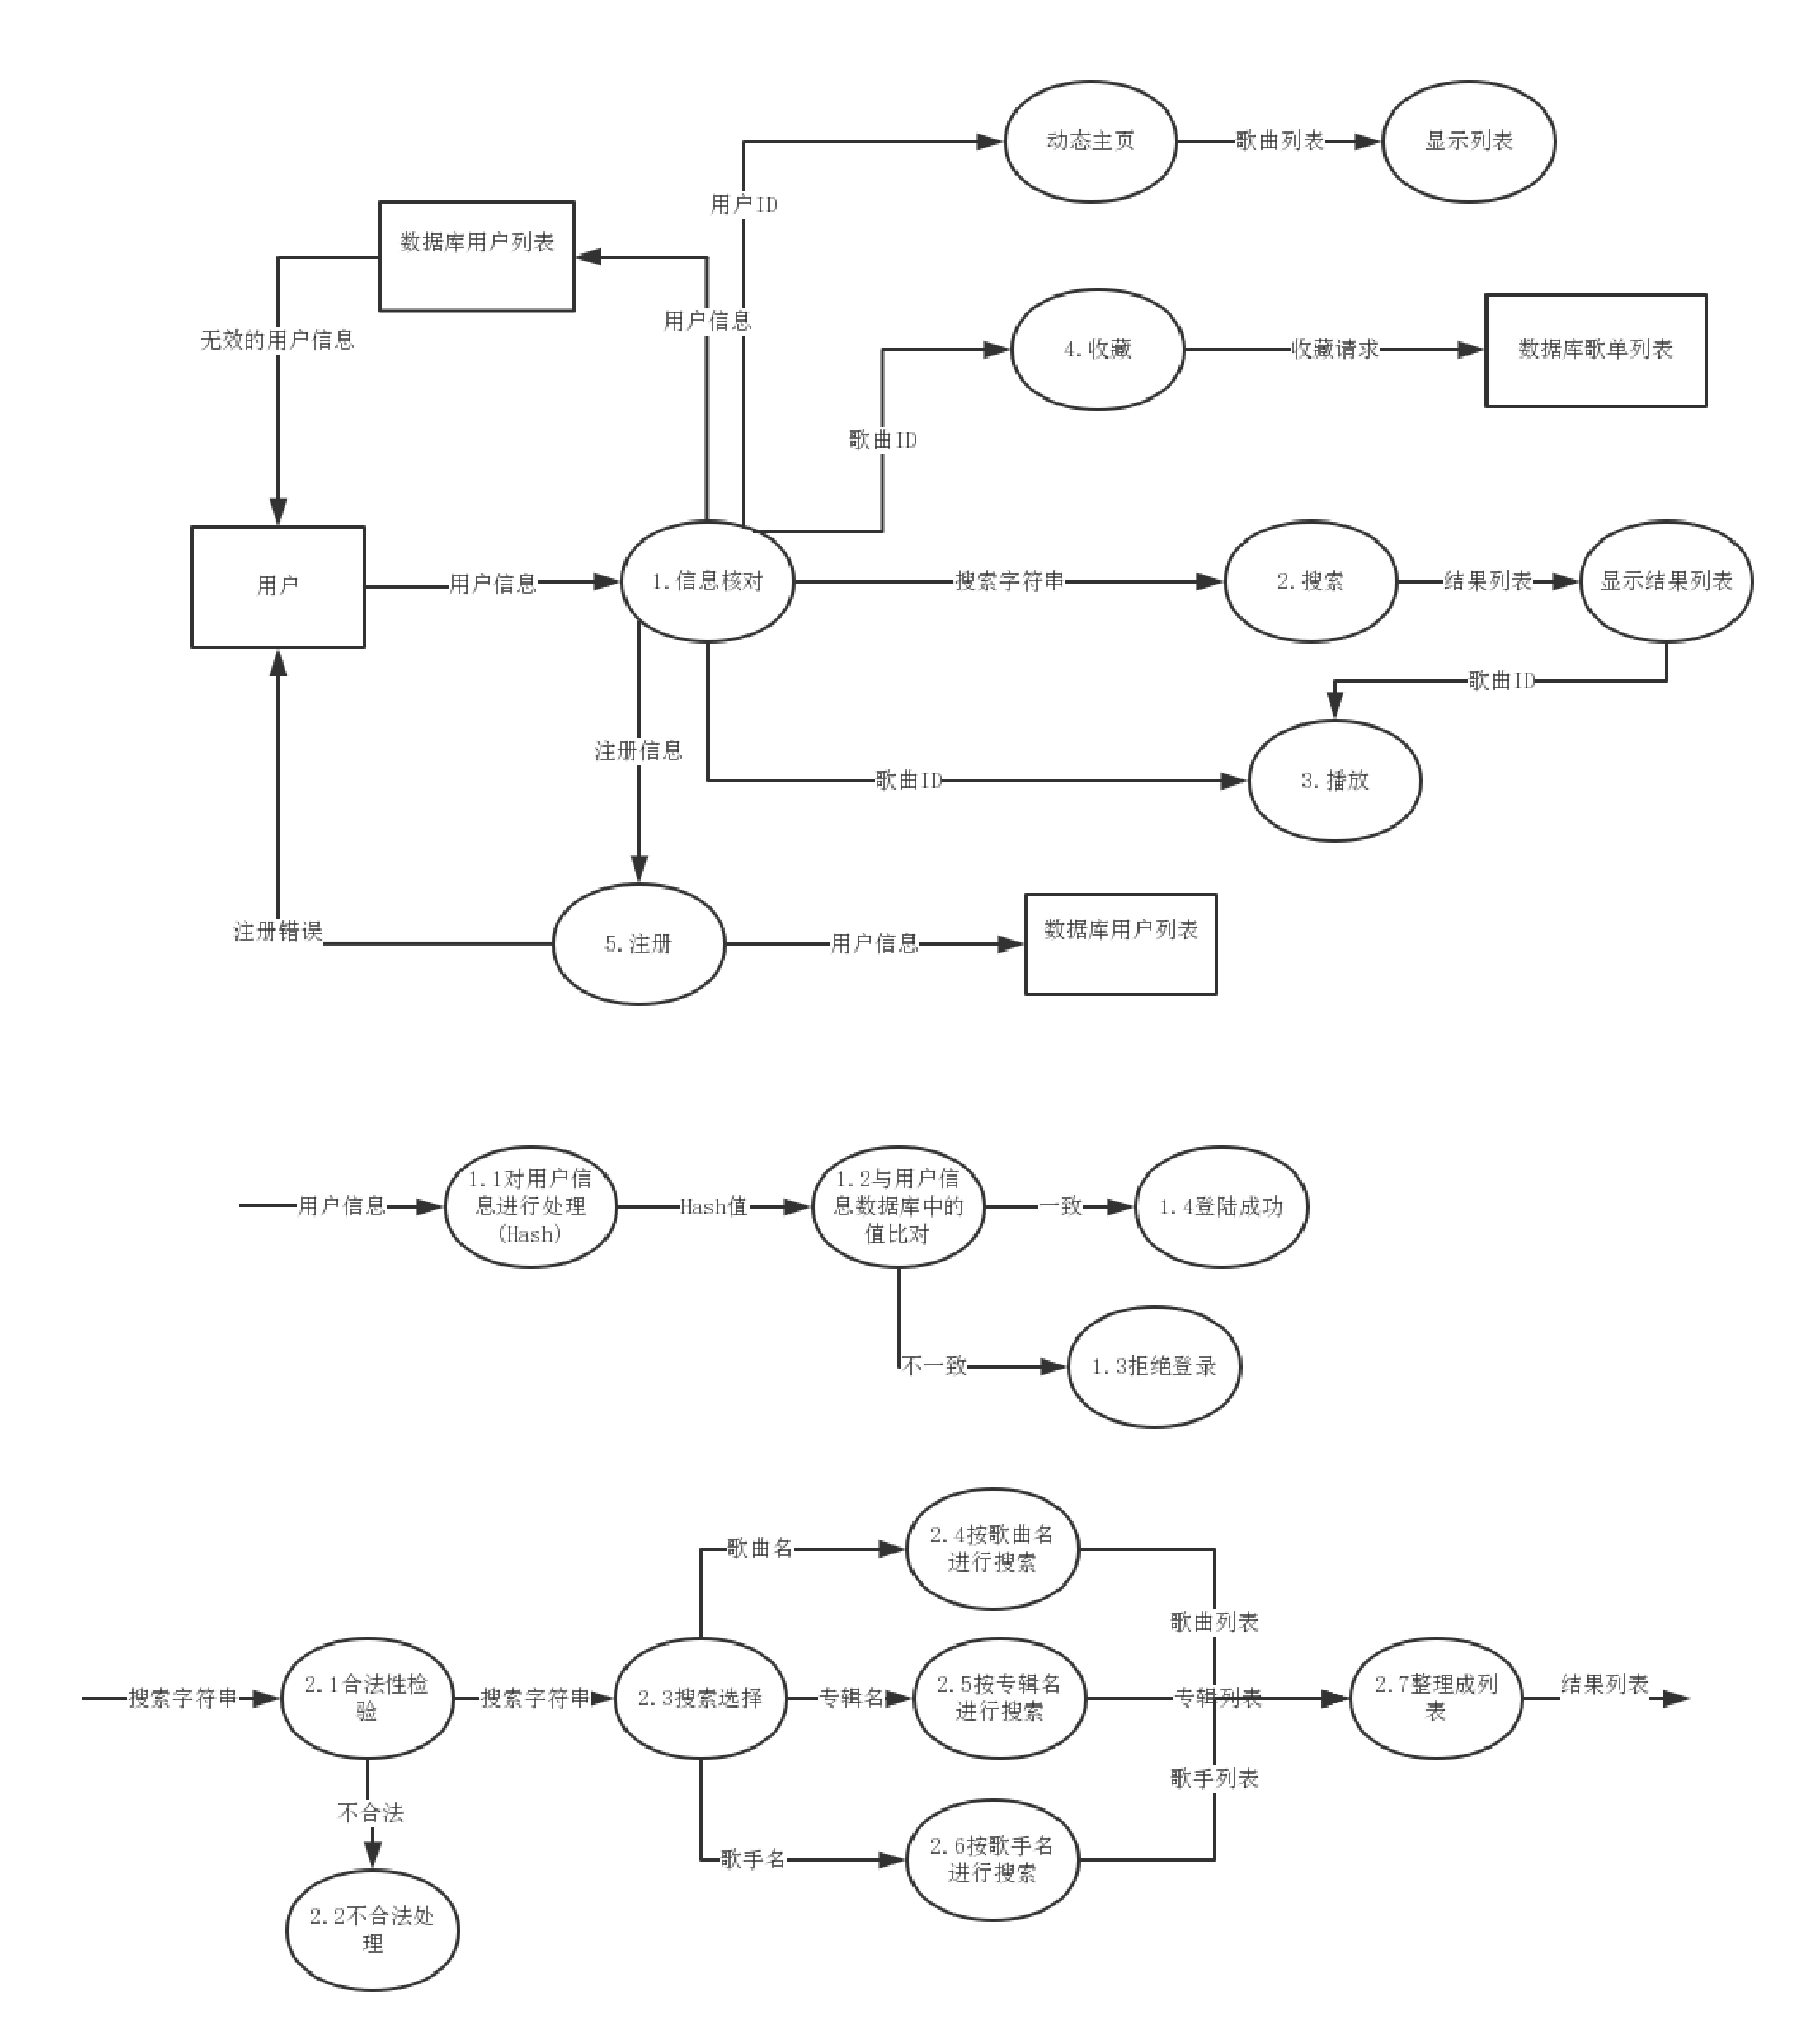
\includegraphics[width=10cm]{lv-1}
	\caption{顶层数据流图} \label{fig:figure13}
\end{figure}

\begin{figure}[ht]
	\centering
	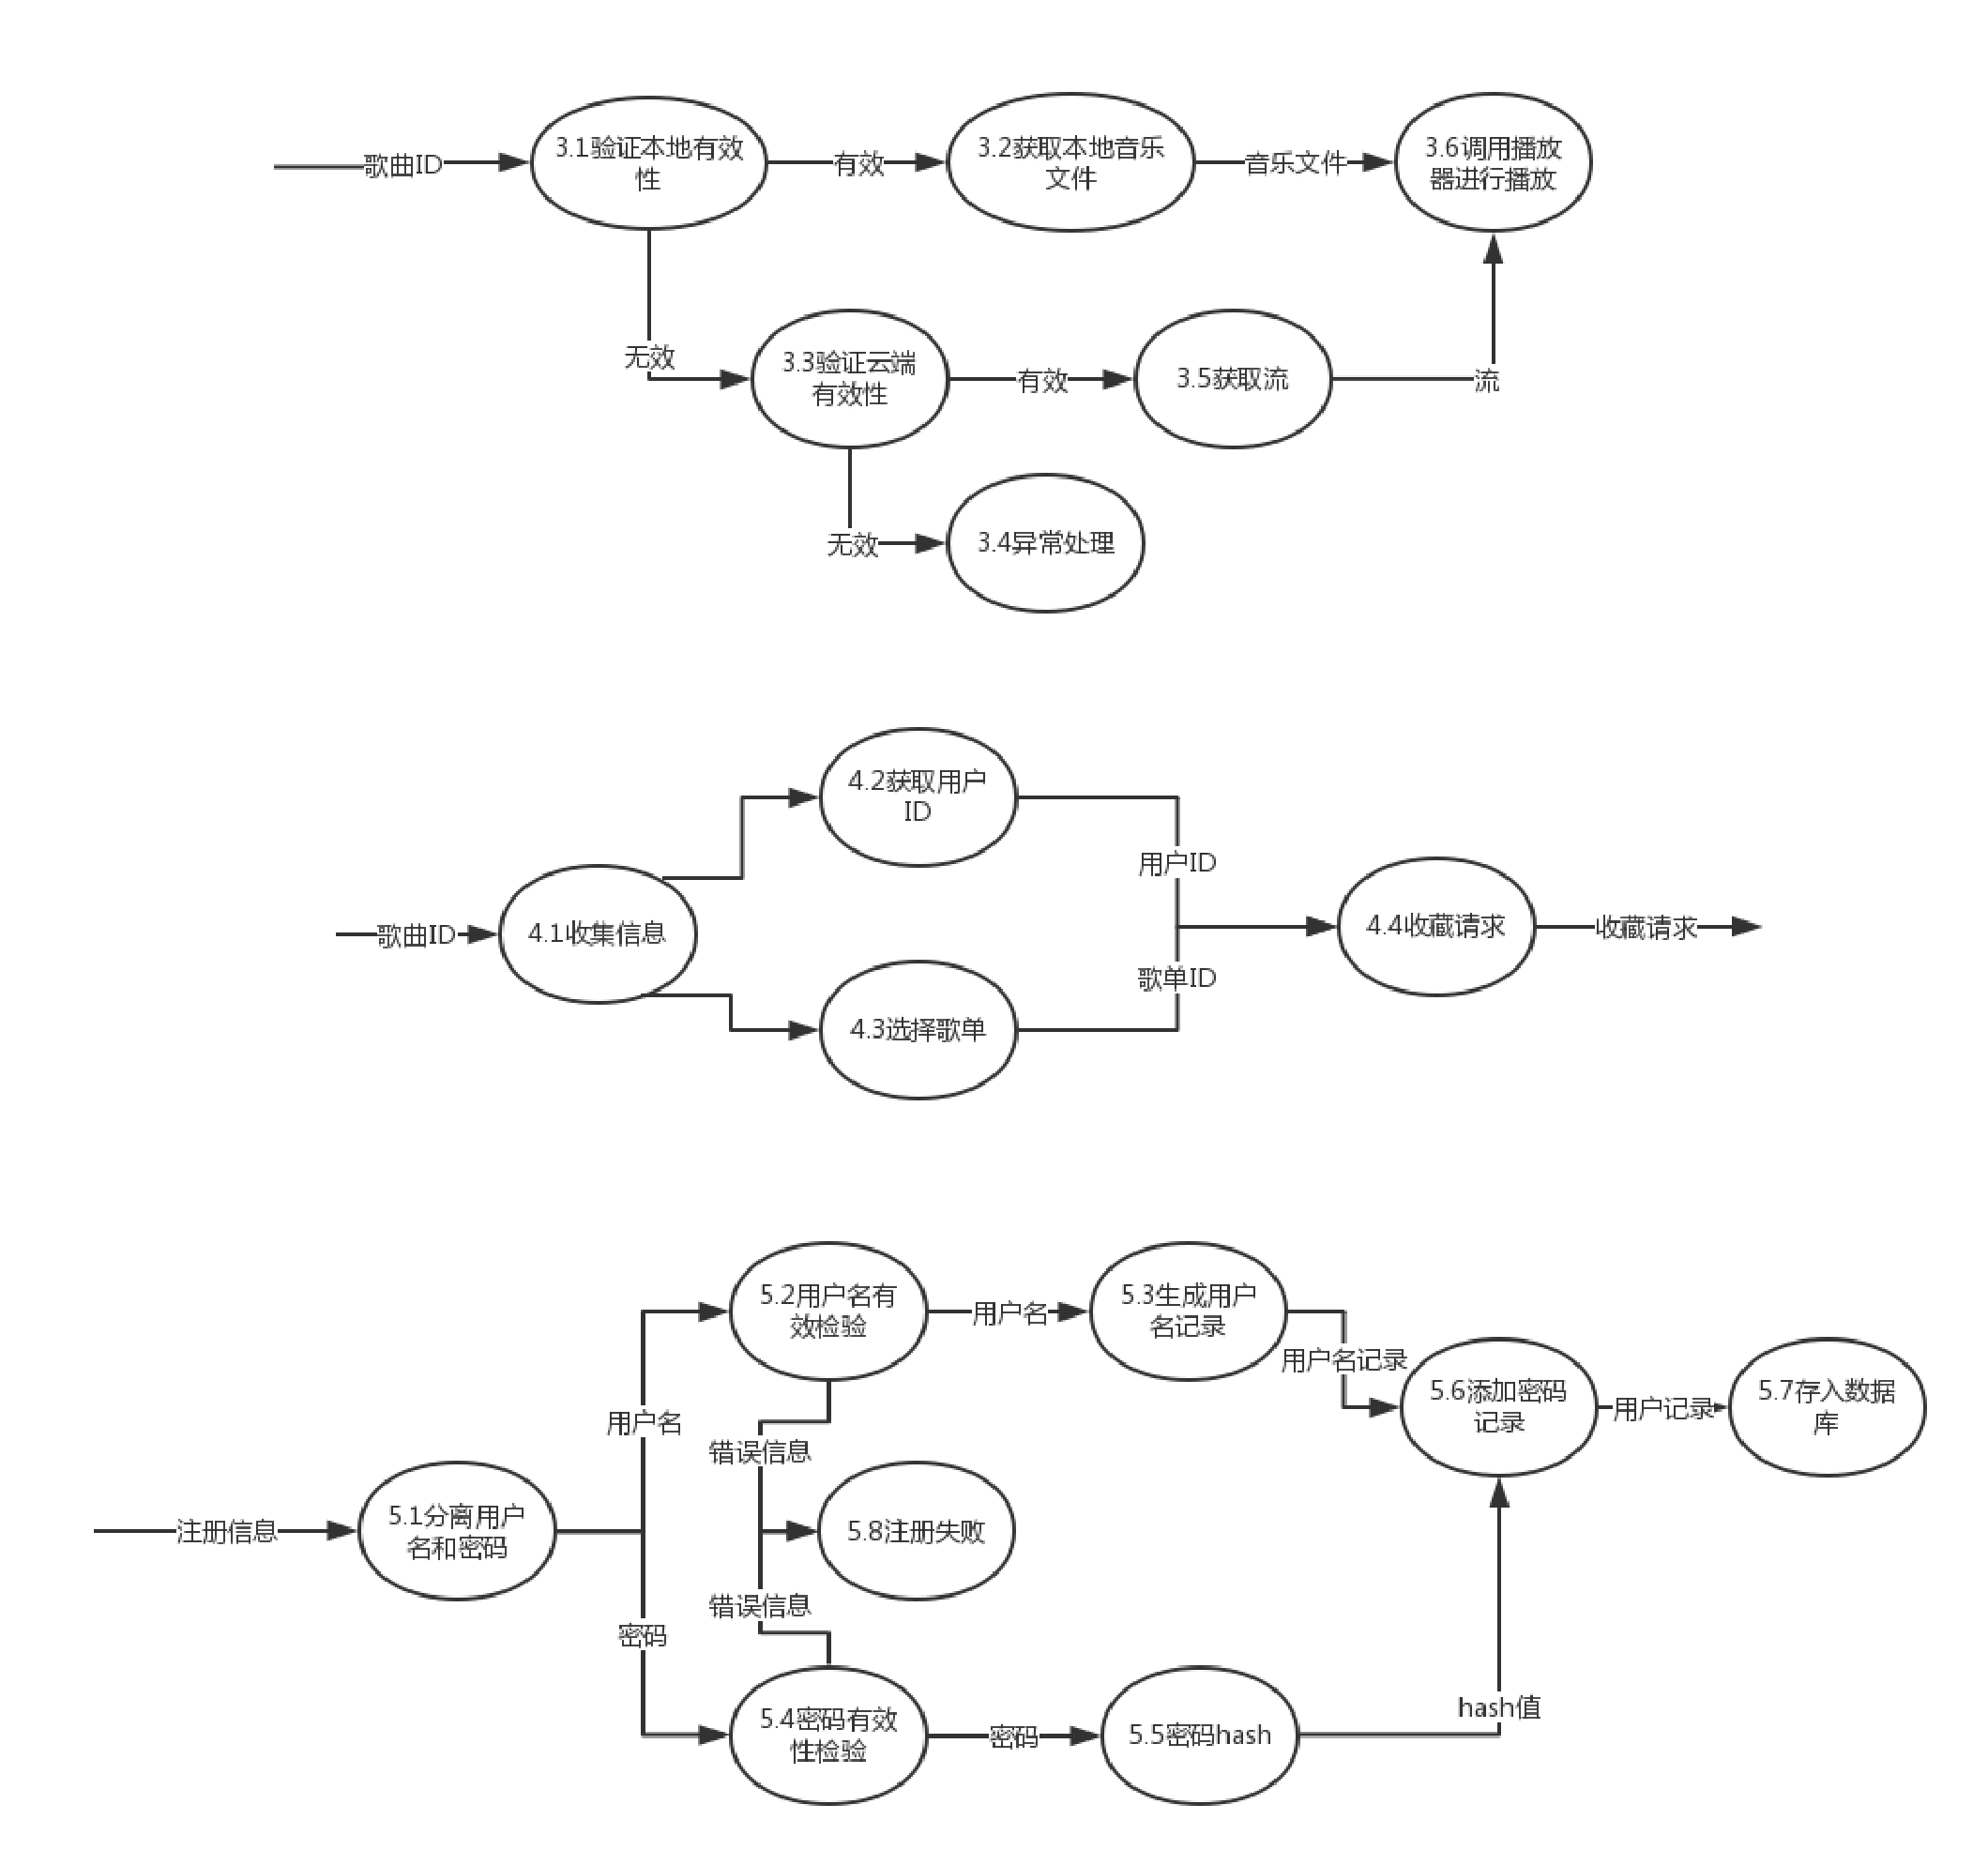
\includegraphics[width=10cm]{lv-1-2}
	\caption{顶层数据流图} \label{fig:figure14}
\end{figure}

\section{数据字典}
\subsection{数据流说明}

\subsubsection{用户信息}

用户信息包含用户名,密码两个内容,用于登录操作中

\subsubsection{歌曲ID}

歌曲ID是用来区分歌曲的唯一特征名称,为1-99长度的Unicode字符串

\subsubsection{专辑ID}

专辑ID是用来区分专辑的唯一特征名称,为1-99长度的Unicode字符串

\subsubsection{歌单ID}

歌单ID是用来区分歌单的唯一特征名称,为1-99长度的Unicode字符串

\subsubsection{搜索字符串}

搜索字符串用于搜索,为1-99长度的Unicode字符串

\subsubsection{歌曲列表}

歌曲列表是一个只包含歌曲ID的列表,该列表是变长的.

\subsubsection{结果列表}

结果列表是搜索结果的返回值,他是一个包含了专辑列表,歌曲列表,歌手列表的列表.


\subsection{加工说明}

\subsubsection{1.1对用户信息进行处理(Hash)}

调用特定的Hash函数,以用户名,密码为输入,返回一个特定的Hash值

\subsubsection{1.2与用户信息数据库中的值比对}

比较输入的Hash值和数据库中对应用户名的条目保存的Hash值进行比对,判断是否一致

\subsubsection{1.3拒绝登录}

返回给客户端一个失败的登录信息

\subsubsection{1.4登陆成功}

返回给客户端一个成功的登录信息并包含一个代表成功登陆的特征码

\subsubsection{2.1合法性检验}

检查搜索字符串内是否包含不合法的字符,并检验字符串长度是否符合要求

\subsubsection{2.2不合法处理}

在客户端内显示错误信息,请求失败

\subsubsection{2.3搜索选择}

将搜索请求分别发送至歌曲,专辑,歌手数据库中进行搜索

\subsubsection{2.4 2.5 2.6}

分别在数据库内执行搜索操作

\subsubsection{2.7整理成列表}

将来自三个数据库的搜索结果整合到一个列表中

\subsubsection{3.1验证本地有效性}

查询本地歌曲数据库中是否保存了目标的歌曲,并且歌曲文件也必须在本地保存.如果都满足,则认为本地有效;否则为无效

\subsubsection{3.2获取本地音乐文件}

查询本地歌曲数据库,获得输入的歌曲ID对应的本地音乐文件的位置

\subsubsection{3.3验证云端有效性}

将歌曲ID发向云端,云端检查该歌曲是否保存在数据库中,如果不在,认为云端无效.否则为有效,向客户端发回响应.

\subsubsection{3.4异常处理}

云端歌曲无效,向客户端发送错误信息

\subsubsection{3.5获取流}

客户端项云端发出请求,云端返回一个流媒体连接.

\subsubsection{3.6调用播放器进行播放}

调用系统API,对获得的流/媒体文件进行播放


